\documentclass{report}

\usepackage{graphicx} % Required for inserting images
\usepackage{amsmath,amssymb}
\usepackage[ruled,vlined]{algorithm2e}

\usepackage{url}

\usepackage{pgfplots}
\pgfplotsset{compat=1.18} % Use a recent compatibility version
\usetikzlibrary{arrows.meta} % For nicer arrows


\usepackage{xcolor}
\usepackage{listings}


\definecolor{maincolor}{HTML}{1E90FF}


\usepackage[colorlinks=true,
            urlcolor=maincolor]{hyperref}


\begin{document}


\subsection{XOR}
Lo \textbf{XOR} (\textit{eXclusive OR}) è un operatore booleano binario la cui tabella di verità è la seguente:

\begin{center}
\begin{table}[h]
\centering
\begin{tabular}{c|c|c}
A & B & XOR(A, B) \\
\hline
0 & 0 & 0         \\
0 & 1 & 1         \\
1 & 0 & 1         \\
1 & 1 & 0         \\
\end{tabular}
\end{table}
\end{center}

Per ricordarla a memoria, basta sapere che, se A e B sono diversi, lo XOR restituisce 1; altrimenti, se sono uguali, restituisce 0.

Ci interessano in particolare le seguenti proprietà dello XOR:

\begin{equation*} (A \oplus B) \oplus B = A \end{equation*}

\begin{equation*} A \oplus 0 = A \end{equation*}

dove $\oplus$ è il simbolo dello XOR. In realtà, queste proprietà sono tutto ciò che ci serve per comprendere il nostro algoritmo crittografico, quindi passiamo ad analizzarne il funzionamento.















\newpage
\subsection{Funzionamento}
L'algoritmo \textbf{OTP} inizia generando una chiave lunga almeno quanto il messaggio da cifrare. La chiave può assumere qualsiasi forma, purché sia privata e nessuno la conosca. Dopo la generazione della chiave, è sufficiente XORarla con il messaggio che vogliamo inviare:  

\begin{equation*}
    C = M \oplus K 
\end{equation*}

dove \(C\) è il messaggio cifrato (\textit{Crypted message}), \(M\) è il messaggio originale (\textit{Message}) e \(K\) è la chiave (\textit{Key}).  

Una volta inviato il messaggio, il destinatario può semplicemente applicare l'operazione XOR tra il messaggio ricevuto e la chiave per recuperare il messaggio originale:  

\begin{equation*}
   C \oplus K
\end{equation*}

Per capire perché il metodo funziona, sostituiamo l'equazione precedente (\(C = M \oplus K\)):  

\begin{equation*}
    (M \oplus K) \oplus K
\end{equation*}

Utilizzando la proprietà dello XOR, otteniamo:  

\begin{equation*}
    M = (M \oplus K) \oplus K 
\end{equation*}

In questo modo, applicando l'operazione XOR, recuperiamo esattamente il messaggio originale.  














\begin{figure}[h]
    \centering
    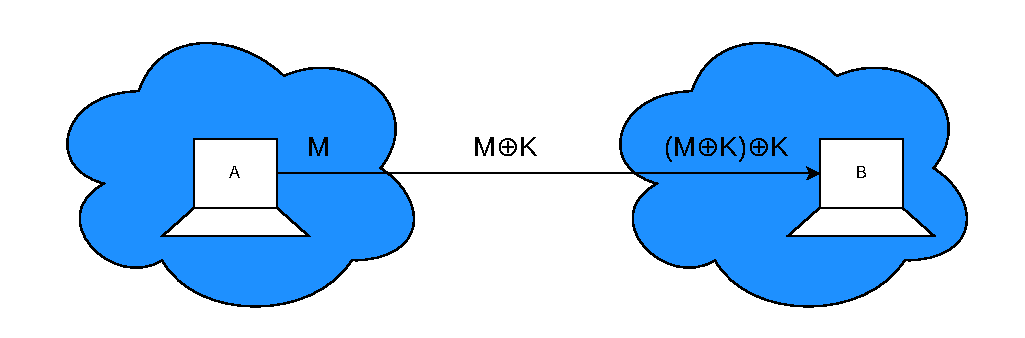
\includegraphics[width=0.9\linewidth]{logos/3_1cripto.pdf}
\end{figure}


\subsubsection{Considerazioni}

Questo algoritmo, però, non si occupa della condivisione sicura della chiave. Per questo scopo si può utilizzare l'algoritmo \textbf{Diffie-Hellman}, che è progettato proprio per condividere chiavi private in modo sicuro.  

La forza e la bellezza di questo algoritmo risiedono nel fatto che è \textbf{completamente sicuro}: è stato infatti dimostrato matematicamente che è impossibile decifrare il messaggio cifrato (\(M \oplus K\)) senza conoscere la chiave. L'\textbf{OTP} è, infatti, l'unico algoritmo \textbf{impossibile da decifrare} e completamente sicuro che conosciamo al momento. L'unico metodo per indovinare il messaggio è tentare casualmente e sperare in un colpo di fortuna.  

Ovviamente, non è tutto oro ciò che luccica: se fosse davvero perfetto, useremmo solo questa tecnica e saremmo al 100\% sicuri. Tuttavia, come vedremo, questo algoritmo presenta un problema non da poco.  




\subsection{Crackabilità}
Il problema di questa tecnica risiede nel nome: \textbf{ONE TIME Pad}. Ovvero, questa tecnica si può usare \textbf{una sola volta} con la stessa chiave. Questo è un requisito fondamentale, perché qualora una chiave venga usata più di una volta, tramite varie tecniche si può estrapolare la chiave e i messaggi, almeno parzialmente.  

Questo accade perché, dati due messaggi in chiaro (\(\mathbf{M_1}\), \(\mathbf{M_2}\)), una chiave privata (\(\mathbf{K}\)) e le loro combinazioni cifrate (\(\mathbf{C_1}\), \(\mathbf{C_2}\)):  

\begin{equation*}
    C_1 = M_1 \oplus K 
\end{equation*}
\begin{equation*}
    C_2 = M_2 \oplus K    
\end{equation*}

Supponiamo di aver intercettato i messaggi cifrati: possiamo applicare l'operazione XOR tra di loro:  

\begin{equation*}
    C_1 \oplus C_2
\end{equation*}

Riscriviamo l'espressione sostituendo i valori di \(C_1\) e \(C_2\):  

\begin{equation*}
    C_1 \oplus C_2 = (M_1 \oplus K ) \oplus (M_2 \oplus K)
\end{equation*}

Ora, grazie alla proprietà associativa dello XOR, possiamo riorganizzare i termini:  

\begin{equation*}
    C_1 \oplus C_2 = (M_1 \oplus M_2 ) \oplus (K \oplus K)
\end{equation*}

Poiché \(K \oplus K = 0\), otteniamo:  

\begin{equation*}
    C_1 \oplus C_2 = (M_1 \oplus M_2 ) \oplus 0
\end{equation*}

Infine, ricordando che \(X \oplus 0 = X\), il risultato finale è:  

\begin{equation*}
    C_1 \oplus C_2 = M_1 \oplus M_2 
\end{equation*}




Dopo tutti questi passaggi, abbiamo scoperto che la XOR tra i du.



e messaggi cifrati è uguale alla XOR dei due messaggi in chiaro. In questo modo, siamo riusciti a "rimuovere" la chiave. Chiaramente, con la XOR dei messaggi in chiaro, comunque non riusciamo a decriptarli, ma possiamo dedurre alcune parti. Infatti, esistono alcuni algoritmi, come \textbf{crib drag}, che, dati alcuni messaggi cifrati, possono decifrare parti dei messaggi e della chiave. Questi algoritmi sono particolarmente complessi e sfruttano certi pattern nelle frasi (come banalmente gli spazi, oppure gli articoli nelle varie lingue) e anche degli \textbf{attacchi con dizionario} (dictionary attack). Per capirli bene e in maniera pratica, consiglio di scaricare i seguenti script Python: \url{https://github.com/CameronLonsdale/MTP}. Inoltre, per gli amanti del rap, vi lascio un esempio divertente per cercare di capire quale canzone è: \url{https://github.com/AlexBro98LoVero/Dispense/blob/main/Giochi/3_1_mtptxt}
\end{document}